
%\documentclass{report}
\documentclass{article}
%\documentclass{scrartcl}

%\usepackage{mslapa}
\usepackage{hyperref}
\usepackage{amsmath}
\usepackage{graphicx}
\usepackage{ulem}
\usepackage{vmargin}
\usepackage{tabularx}
\usepackage{sectsty}
\usepackage{pbox}
\usepackage{bigstrut}
\usepackage{enumerate}
\usepackage{listings}
\usepackage{parskip}   % space paragraphs but dont indent
\usepackage{verbatim}  % \verbatiminput{file}
\usepackage{gensymb}
\usepackage{color}

\usepackage{natbib}

%\setpapersize{USletter}
%\sectionfont{\normalsize}
%\subsectionfont{\normalsize}
\setmarginsrb{1.0in}{1.0in}{1.0in}{1.0in}{0in}{0.25in}{0in}{0.20in}

% configure \bigstrut size
% This configures spacing above and below rows in a tabularx.
\renewcommand{\bigstrutjot}{2.0\jot}

\providecommand{\e}[1]{\ensuremath{\times 10^{#1}}}

\raggedright

\begin{document}

% {{{ Title Page

\centerline{\Large \textbf{Bus Communications Over SPI}}
\vspace{2em}
\centerline{\small \textbf{EECE 344, Spring 2012, CSU Chico}}
\vspace{0.5em}
\centerline{\small \textbf{Jeremiah Mahler \href{mailto:jmahler@mail.csuchico.edu}{jmahler@mail.csuchico.edu}}}
\vspace{2em}
\thispagestyle{empty}

% }}}

%\tableofcontents
%\pagebreak

% {{{ Introduction
\section{Introduction}

A bus is used to allow communication with multiple devices
over a shared set of wires.
The Serial Peripheral Interface (SPI) provides a means
for transferring data between two devices.
This project shows how an ARM board can communicate over
SPI to a CPLD which defines a bus.
Figure \ref{fig:bus} gives an overview.

There are two main components used in this project which
will be referred to in an abbreviated form throughout this document.
The term "ARM" will refer to the ARM STM32L Discovery\cite{UM1079} board.
And the term "CPLD" will refer to the Lattice MachXO\cite{EB66}
CPLD board.
This project is specific to these development boards although it
may be possible to substitute others with some modification.

\begin{figure}[hbp]
\center
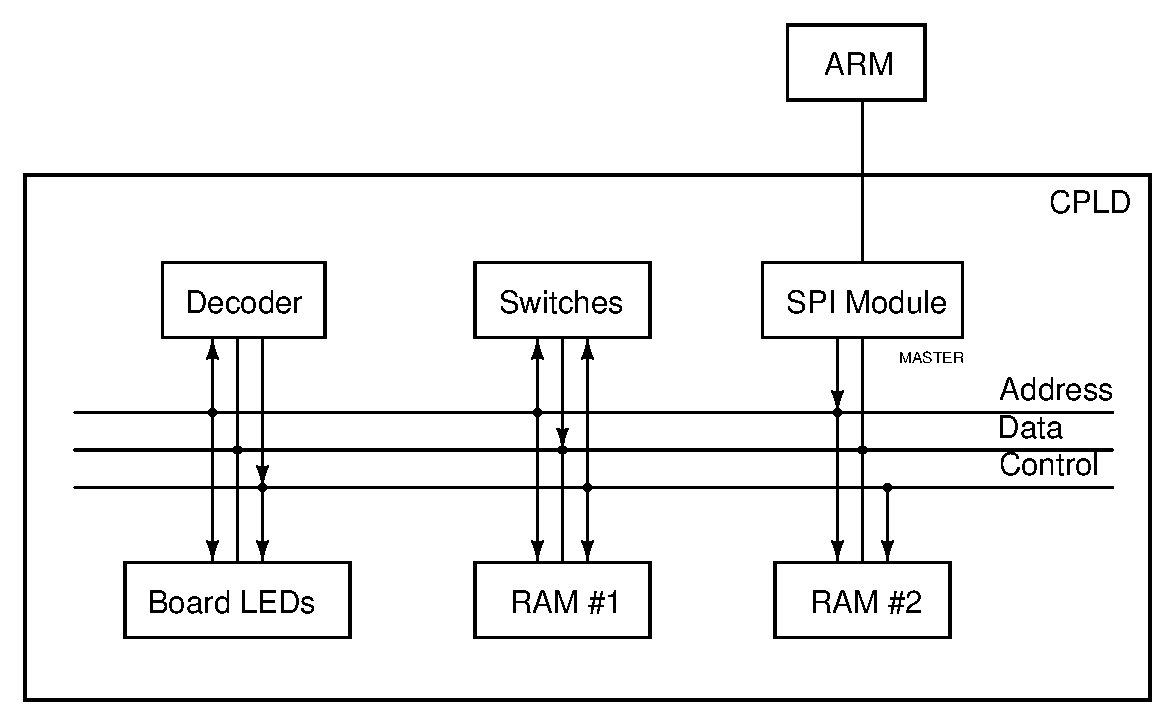
\includegraphics[scale=0.7]{figures/schematics/BUS}
\caption{Conceptual overview of bus and related components.
The ARM is only able to communicate with the bus through the SPI
module.
And all the components which are on the bus are controlled by the
CPLD.
Arrows designate input/output and if there are none it is bidirectional.
Refer to table \ref{tbl:memmap} for the specific address used.
}
\label{fig:bus}
\end{figure}

\begin{table}[hbp]
\center
\begin{tabular}{|l|l|}
    \hline
    \multicolumn{2}{|c|}{\textbf{Memory Map}} \\
    \hline
    address (hex) & name \\
    \hline
    0x74 & switches \\
    0x6C & bar leds \\
    0x50 - 0x5F & RAM \#2 \\
    0x2F & board leds \\
    0x00 - 0x0F & RAM \#1 \\
    \hline
\end{tabular}
\caption{Device memory map.}
\label{tbl:memmap}
\end{table}

%\begin{figure}[hbp]
%\center
%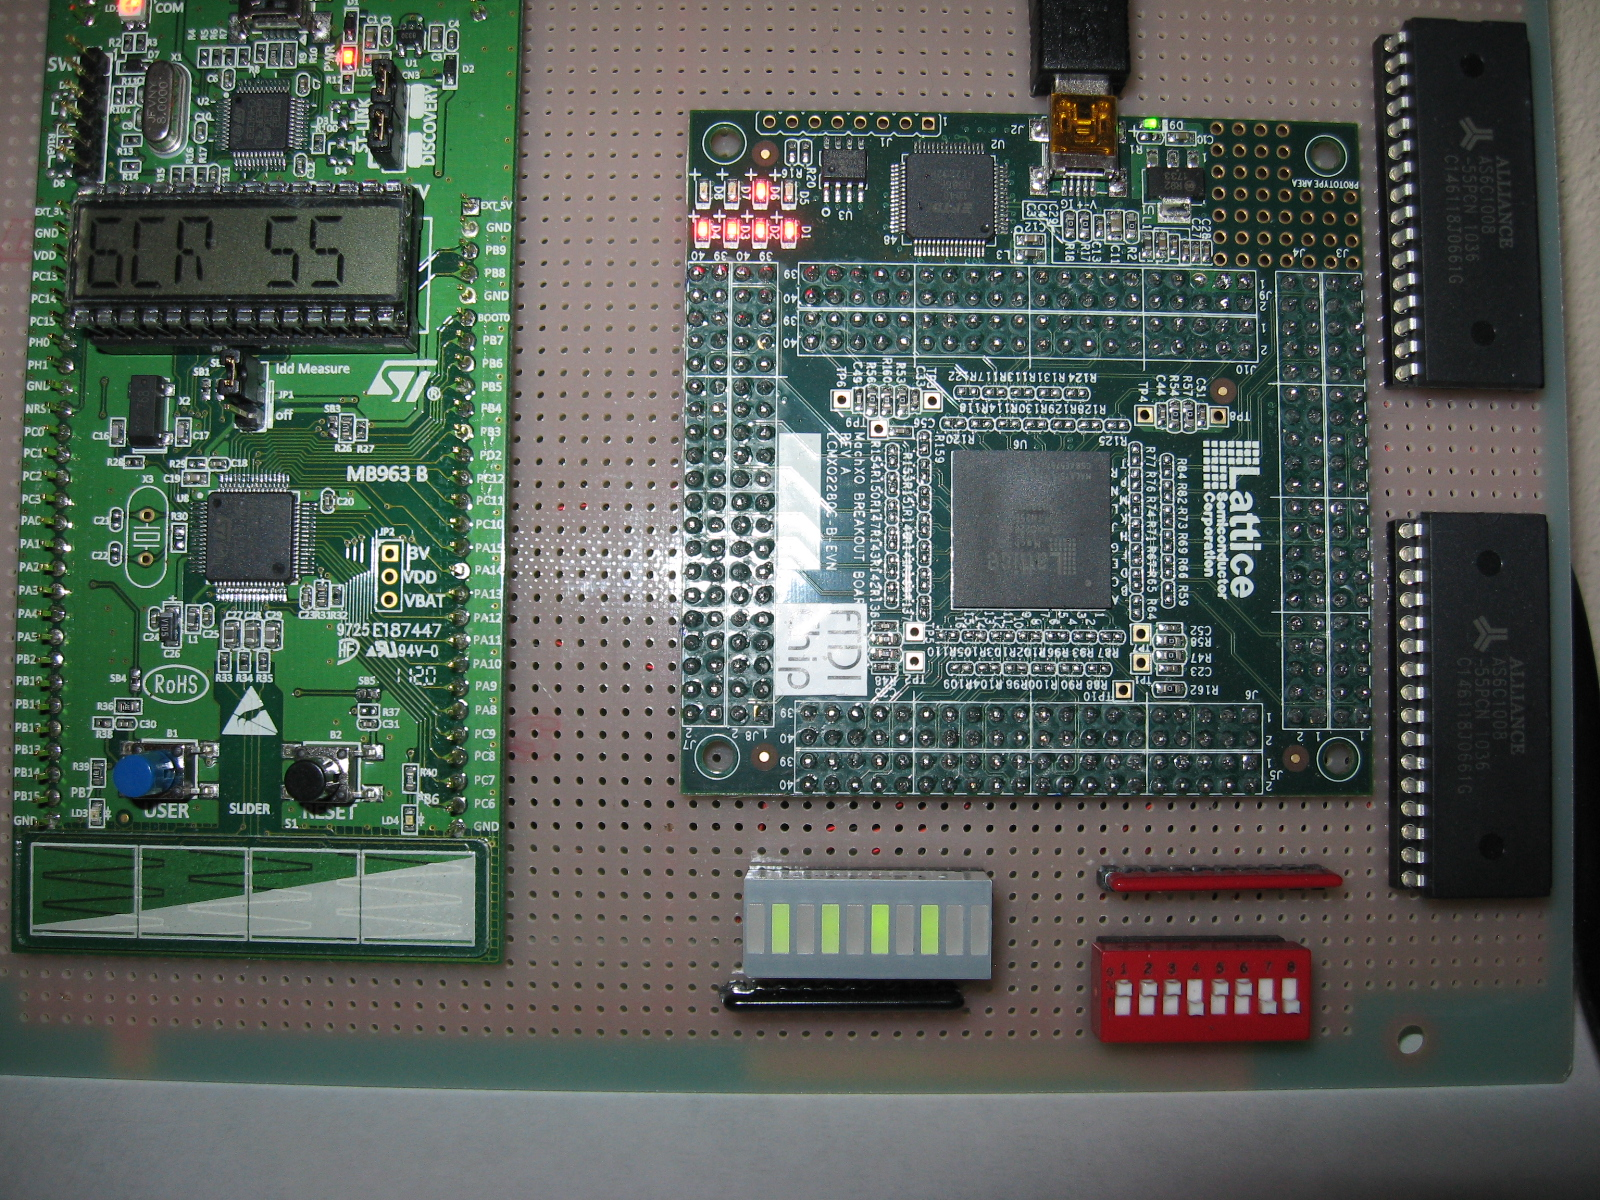
\includegraphics[scale=0.3]{figures/imgs/IMG_3001}
%\caption{Picture of assembled board.}
%\end{figure}

% }}}

% {{{ Bus Interface
\section{Bus Interface}
\label{sec:bus}

Before we can communicate with the bus over SPI we need
to define how the bus itself works.
There are two main operations that must be supported: read and write.

For a read cycle the first step is to drive the address value.
Then the device is enabled and some time later read is enabled.
At this point the device knows it should it should drive the
data but it will take some time for it to become valid.
After the data has been read the cycle is finished and the device is disabled.
Figure \ref{fig:bus_cycle} (a) shows this read cycle.

For a write cycle the first step is to drive the address value.
Then the device is enabled and some time later write is enabled.
At this point the data should be driven by the bus master
but it will take some time to become valid.
At the end of the write strobe, before it is disabled,
the data should be latched by the device.
Figure \ref{fig:bus_cycle} (b) shows this write cycle.

\begin{figure}
\center

\begin{tabular}{ccc}
\includegraphics[scale=0.7]{figures/bus-timing/read} & \quad &
\includegraphics[scale=0.7]{figures/bus-timing/write} \\
(a) && (b) 
\end{tabular}

\caption{Bus read cycle (a) and write cycle (b).}
\label{fig:bus_cycle}
\end{figure}

A decoder will be used to control the chip enable for all the components
to ensure only one is driving the bus at any given time (Figure \ref{fig:bus}).

% }}}

% {{{ SPI protocol
\section{SPI protocol}
\label{sec:spi}

Since the ARM cannot connect directly to the bus the SPI
is used as a communication channel.
The read and write operations that need to be performed
require a minimum of two bytes.
A read, for example, would send the address in the first transaction.
And in the second transaction the data read would be returned.
A write is similar except that for the second transaction the
data to be written is sent.
The format of the bytes for each transaction is shown in Table \ref{tbl:spiformat}.

\begin{table}[hbp]
\center
\begin{tabular}{|c|c|c|}
    \multicolumn{1}{l}{8} & \multicolumn{1}{l}{7} & \multicolumn{1}{r}{1} \\
\hline
rw bit & \multicolumn{2}{|c|}{address} \\
\hline
\multicolumn{3}{|c|}{data} \\
\hline
\end{tabular}
\caption{Format of two byte SPI transactions.}
\label{tbl:spiformat}
\end{table}

Note, this implementation is configured with the SPI settings
shown in Table \ref{tbl:spi}.
Both the ARM and the CPLD must use these same settings in order
to work properly with each other.

\begin{table}
\center
\begin{tabular}{|l|l|}
	\hline
	option & value \\
	\hline
	MSB & first \\
	CPOL & 0 \\
	CPHA & 0 \\
	NSS & slave select\\
	\hline
\end{tabular}
\caption{SPI configuration options}
\label{tbl:spi}
\end{table}

In order to perform a read/write the timing of the bus operations
(Figure \ref{fig:bus_cycle}) needs to be integrated in to the
timing of SPI operations.
The result is showing in Figure \ref{fig:spi_read} for the
read operation and in Figure \ref{fig:spi_write} for the write.

For a detailed timing diagram of the read and write operations refer
to Figures \ref{fig:spi_read} and \ref{fig:spi_write}.

\begin{figure}
\center
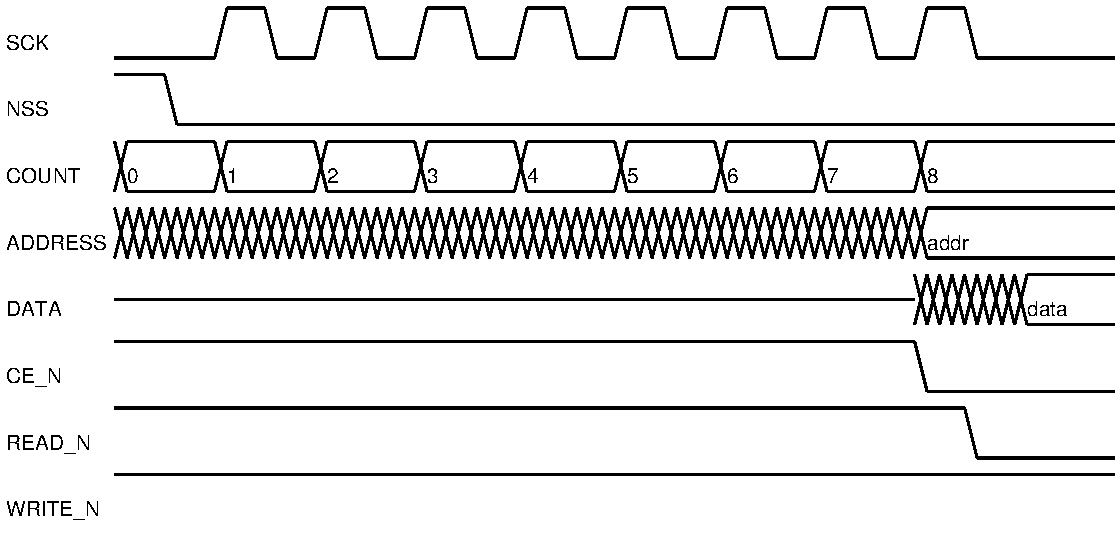
\includegraphics[scale=0.7]{figures/spi_ctl-timing/read-byte1} \\
(a) \\
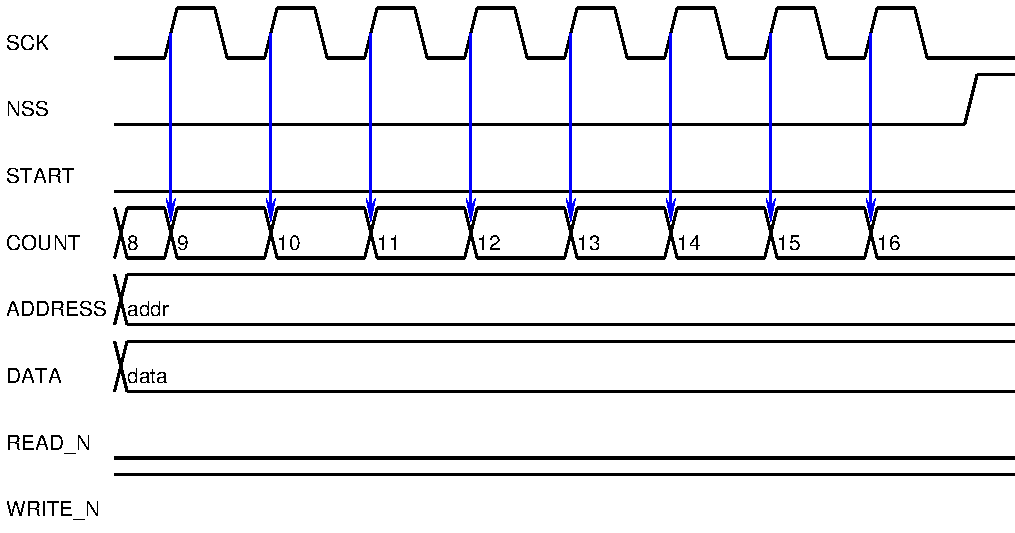
\includegraphics[scale=0.7]{figures/spi_ctl-timing/read-byte2} \\
(b)
\caption{Timing diagram of SPI read cycle.
Part (a) is the first 8-bits and part (b) is the second
8-bits continuing from (a).}
\label{fig:spi_read}
\end{figure}

\begin{figure}
\center
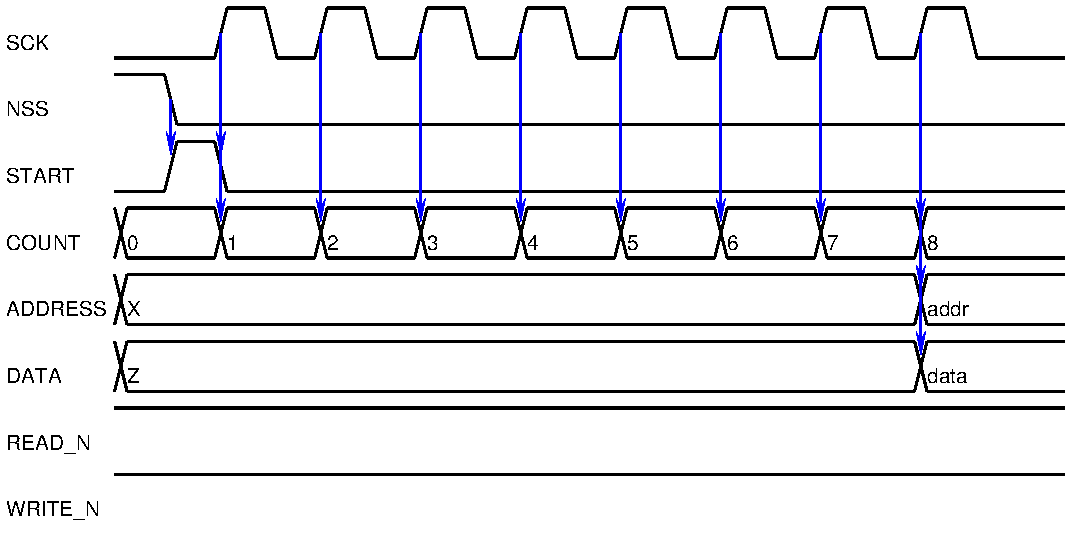
\includegraphics[scale=0.7]{figures/spi_ctl-timing/write-byte1} \\
(a) \\
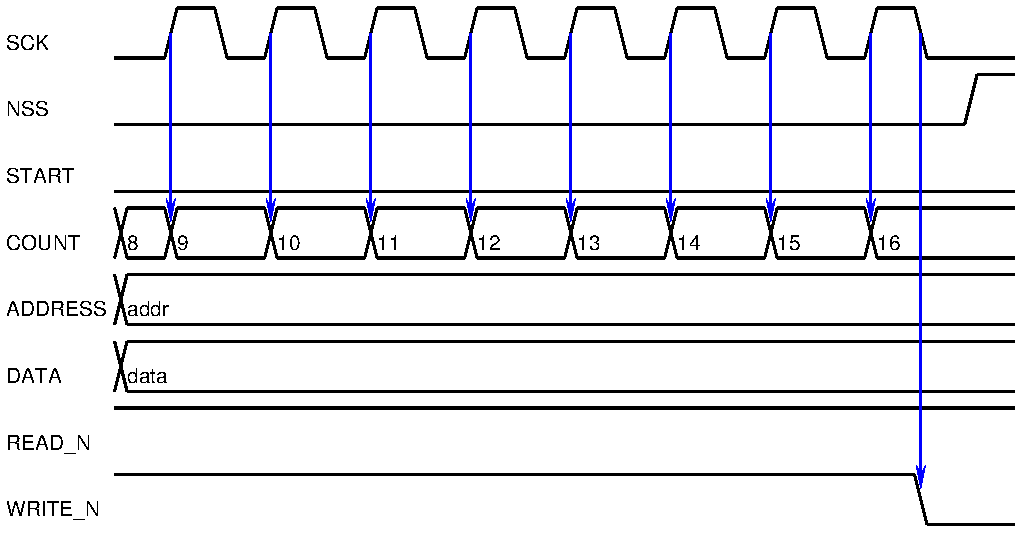
\includegraphics[scale=0.7]{figures/spi_ctl-timing/write-byte2} \\
(b)
\caption{Timing diagram of SPI write cycle.
Part (a) is the first 8-bits and part (b) is the second
continuing from (a).
A write is not initiated until the end of the
second byte because it has to read this byte entirely before it can be written.}
\label{fig:spi_write}
\end{figure}

\clearpage

% }}}

% {{{ User Interface
\section{User Interface}

In order for the user to be able to perform read and write
operations to the bus devices an interface needs to be defined.
The only means of input is using an eight position DIP switch
and a USER button.
Outputs are provided by an LCD, a bar of eight LEDS,
and a group of eight LEDs on board the CPLD.

The bar of LEDs and the group of LEDs on the CPLD both operate
similarly.
They act as an eight bit register which can be read from and written to.
Refer to Table \ref{tbl:memmap} for their specific addresses.

The LCD is the primary means of user feedback.
It instructs the user when to enter a command or data and
it displays the results.
Figure \ref{fig:armstate} gives an overview of the states of
the system.

\begin{figure}[hbp]
\center
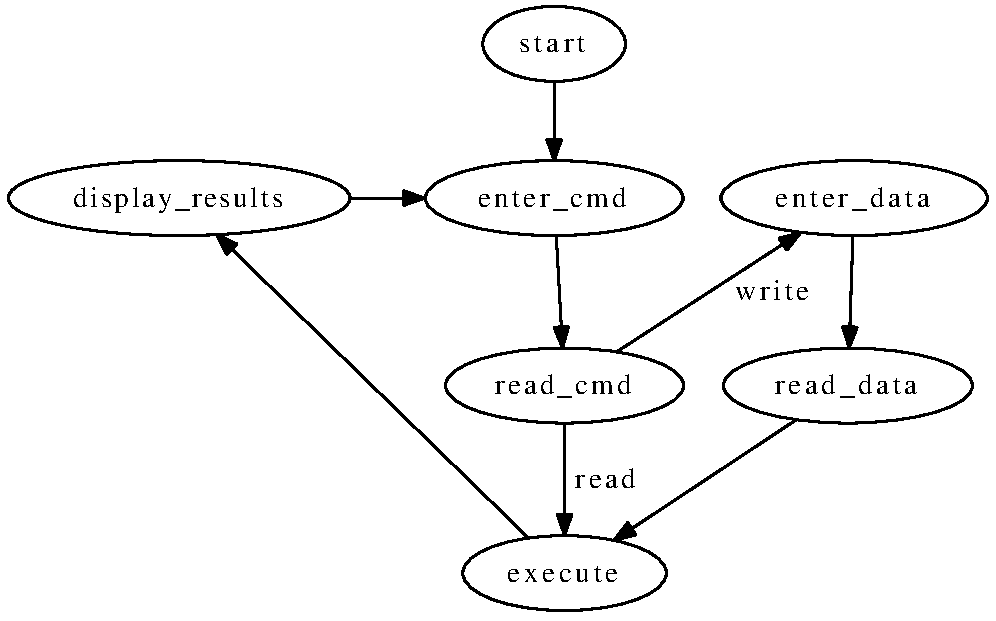
\includegraphics[scale=0.8]{figures/arm-state_diagram/arm-state_diagram}
\caption{State diagram of ARM board operation.
The states 'display\_results', 'enter\_cmd' and 'enter\_data'
wait for the USER button to be pressed before continuing.
'read\_cmd' reads the input switches to get the command (address and rw bit).
If the command is a write 'read\_data' reads the switches again to get the data.
And 'execute' performs the read/write command.
}
\label{fig:armstate}
\end{figure}

As an example the following dialog shows how to read from
the switches.
At each step the USER button is pressed to proceed to the next step.
A value of '--' is used to denote when the switches have no bearing
on the results.

\begin{tabular}{l l l}
LCD & switches & description \\
\hline
\verb+CMD+ & 0xFF & read from address 0x74 (switches) \\
\verb+74 R F4+ & -- & the value 0xF4 was read from address 0x74 \\
\end{tabular}

As another example the following shows how to write to the external LEDs.

\begin{tabular}{l l l}
LCD & switches & description \\
\hline
\verb+CMD+  & 0x6C & write to address 0x6C (bar leds) \\
\verb+DATA+ & 0x35 & the data 0x35 will be written to the address \\
\verb+6C W 35+ & -- & value 0x35 was written to address 0x6C
\end{tabular}

A identical procedure can be performed to read/write to any
of the addresses in the memory map (Table \ref{tbl:memmap}).

% }}}

% {{{ Pin Assignments, Schematics
\section{Pin Assignments, Schematics}
\label{sec:pa}

The pin assignments define all the interconnecting wires
between the ARM, CPLD and other components.

% describe the pin meanings
To locate a pin on the CPLD requires two designations\citep[Pg. 11-14]{EB66}.
The first is the header which has names such as J9, J7, etc.
And the second is the number of the pin.
The board will have pin numbers at the beginning and end of a header
to denote the orientation.

On the CPLD the pins correspond to headers (J9, J7, etc)
and pins within those headers\citep[Pg. 11-14]{EB66}.
The header and pin numbers are printed at the end of each header.

When specifying the pin constraints in Diamond\cite{Diamond}
the header and pin number are not available.
Instead the "Mach XO Ball" must be specified.
And this value is included in the following pin assignments.

The pin assignments are given in Tables
\ref{tbl:ramcommon}, \ref{tbl:rampinsuniq}, \ref{tbl:pins}
as well as the schematic in Figures \ref{fig:ram_to_cpld}, \ref{fig:arm_to_cpld}.

% {{{ RAM common Table
\begin{table}
\center
\begin{tabular}{|l|l|l|l|l|l|l|}
	\hline
	\multicolumn{3}{|c|}{\textbf{RAM}} & \multicolumn{4}{|c|}{\textbf{CPLD}} \\
	\hline
	pin & label & description &  function & Mach XO Ball & Header & Pin \\
	\hline
	12 & A0 & mem\_address & PL17D & L4 & J4 & 36 \\
	\hline
	11 & A1 & mem\_address & PL12D & L2 & J4 & 35 \\
	\hline
	10 & A2 & mem\_address & PL17C & L5 & J4 & 34 \\
	\hline
	9 & A3 & mem\_address & PL12C & K2 & J4 & 33 \\
	\hline
	8 & A4 & mem\_address & PL15C & M2 & J4 & 26 \\
	\hline
	7 & A5 & mem\_address & PL10C & G1 & J4 & 21 \\
	\hline
	6 & A6 & mem\_address & PL10D & H1 & J4 & 23 \\
	\hline
	5 & A7 & mem\_address & PL8D & H3 & J4 & 19 \\
	\hline
	27 & A8 & mem\_address & PL15D & N2 & J4 & 28 \\
	\hline
	26 & A9 & mem\_address & PL11C & J3 & J4 & 29 \\
	\hline
	23 & A10 & mem\_address & PL19A & N4 & J4 & 38 \\
	\hline
	25 & A11 & mem\_address & PL11D & K3 & J4 & 31 \\
	\hline
	4 & A12 & mem\_address & PL8C & G3 & J4 & 17 \\
	\hline
	28 & A13 & mem\_address & PL16D & R2 & J4 & 32 \\
	\hline
	3 & A14 & mem\_address & PL7C & E1 & J4 & 13 \\
	\hline
	31 & A15 & mem\_address & PL7D & F1 & J4 & 15 \\
	\hline
	2 & A16 & mem\_address & PL6D & D1 & J4 & 11 \\
	\hline
	13 & DQ0 & mem\_data & PL7A\_LV\_T & F2 & J3 & 25 \\
	\hline
	14 & DQ1 & mem\_data & PL17A\_LV\_T & K5 & J3 & 32 \\
	\hline
	15 & DQ2 & mem\_data & PL18A\_LV\_T & M5 & J3 & 38 \\
	\hline
	17 & DQ3 & mem\_data & PL9A\_LV\_T & H4 & J3 & 37 \\
	\hline
	18 & DQ4 & mem\_data & PL8A\_LV\_T & G4 & J3 & 31 \\
	\hline
	19 & DQ5 & mem\_data & PL16A\_LV\_T & J4 & J3 & 26 \\
	\hline
	20 & DQ6 & mem\_data & PL15A\_LV\_T & L3 & J3 & 20 \\
	\hline
	21 & DQ7 & mem\_data & PL5A\_LV\_T & B1 & J3 & 19 \\
	\hline
	32 & Vcc & suppy voltage & & & J9 & 5 \\
	\hline
	16 & Vss & ground & & & J3 & 36 \\
	\hline
\end{tabular}
\caption{Pin assignments between RAM chip and the CPLD
which are common to both chips.
See Table \ref{tbl:rampinsuniq} for those pins which are
unique for each chip.
}
\label{tbl:ramcommon}
\end{table}
% }}}

% {{{ RAM unique Table
\begin{table}
\center

\begin{tabular}{|l|l|l|l|l|l|l|l|}
    \hline
	\multicolumn{4}{|c|}{\textbf{RAM \#1}} & \multicolumn{4}{|c|}{\textbf{CPLD}} \\
	\hline
    pin & label & variable & description &  function & Mach XO Ball & Header & Pin \\
    \hline
    30 & CE2 & mem1\_ce2 & chip enable & PL14C & N1 & J4 & 37 \\
	\hline
    22 & CE\# & mem1\_ceh\_n & chip enable & PL19B & N3 & J4 & 40 \\
	\hline
    29 & WE\# & mem1\_we\_n & write enable & PL14D & P1 & J4 & 39 \\
	\hline
    24 & OE\# & mem1\_oe\_n & output enable & PL16C & R1 & J4 & 30 \\
	\hline
\end{tabular}

\vspace{5mm}  

\begin{tabular}{|l|l|l|l|l|l|l|l|}
    \hline
	\multicolumn{4}{|c|}{\textbf{RAM \#2}} & \multicolumn{4}{|c|}{\textbf{CPLD}} \\
	\hline
    pin & label & variable & description &  function & Mach XO Ball & Header & Pin \\
    \hline
    30 & CE2 & mem2\_ce2 & chip enable & PL8B & G5 & J3 & 33 \\
	\hline
    22 & CE\# & mem2\_ceh\_n & chip enable & PL11B & J2 & J3 & 4 \\
	\hline
    29 & WE\# & mem2\_we\_n & write enable & PL19B & H5 & J3 & 39 \\
	\hline
    24 & OE\# & mem2\_oe\_n & output enable & PL18B & M4 & J3 & 40 \\
	\hline
\end{tabular}

\caption{Pin assignments between RAM chip and the CPLD
which are unique to each RAM chip.}
\label{tbl:rampinsuniq}
\end{table}
% }}}

\begin{figure}
\center
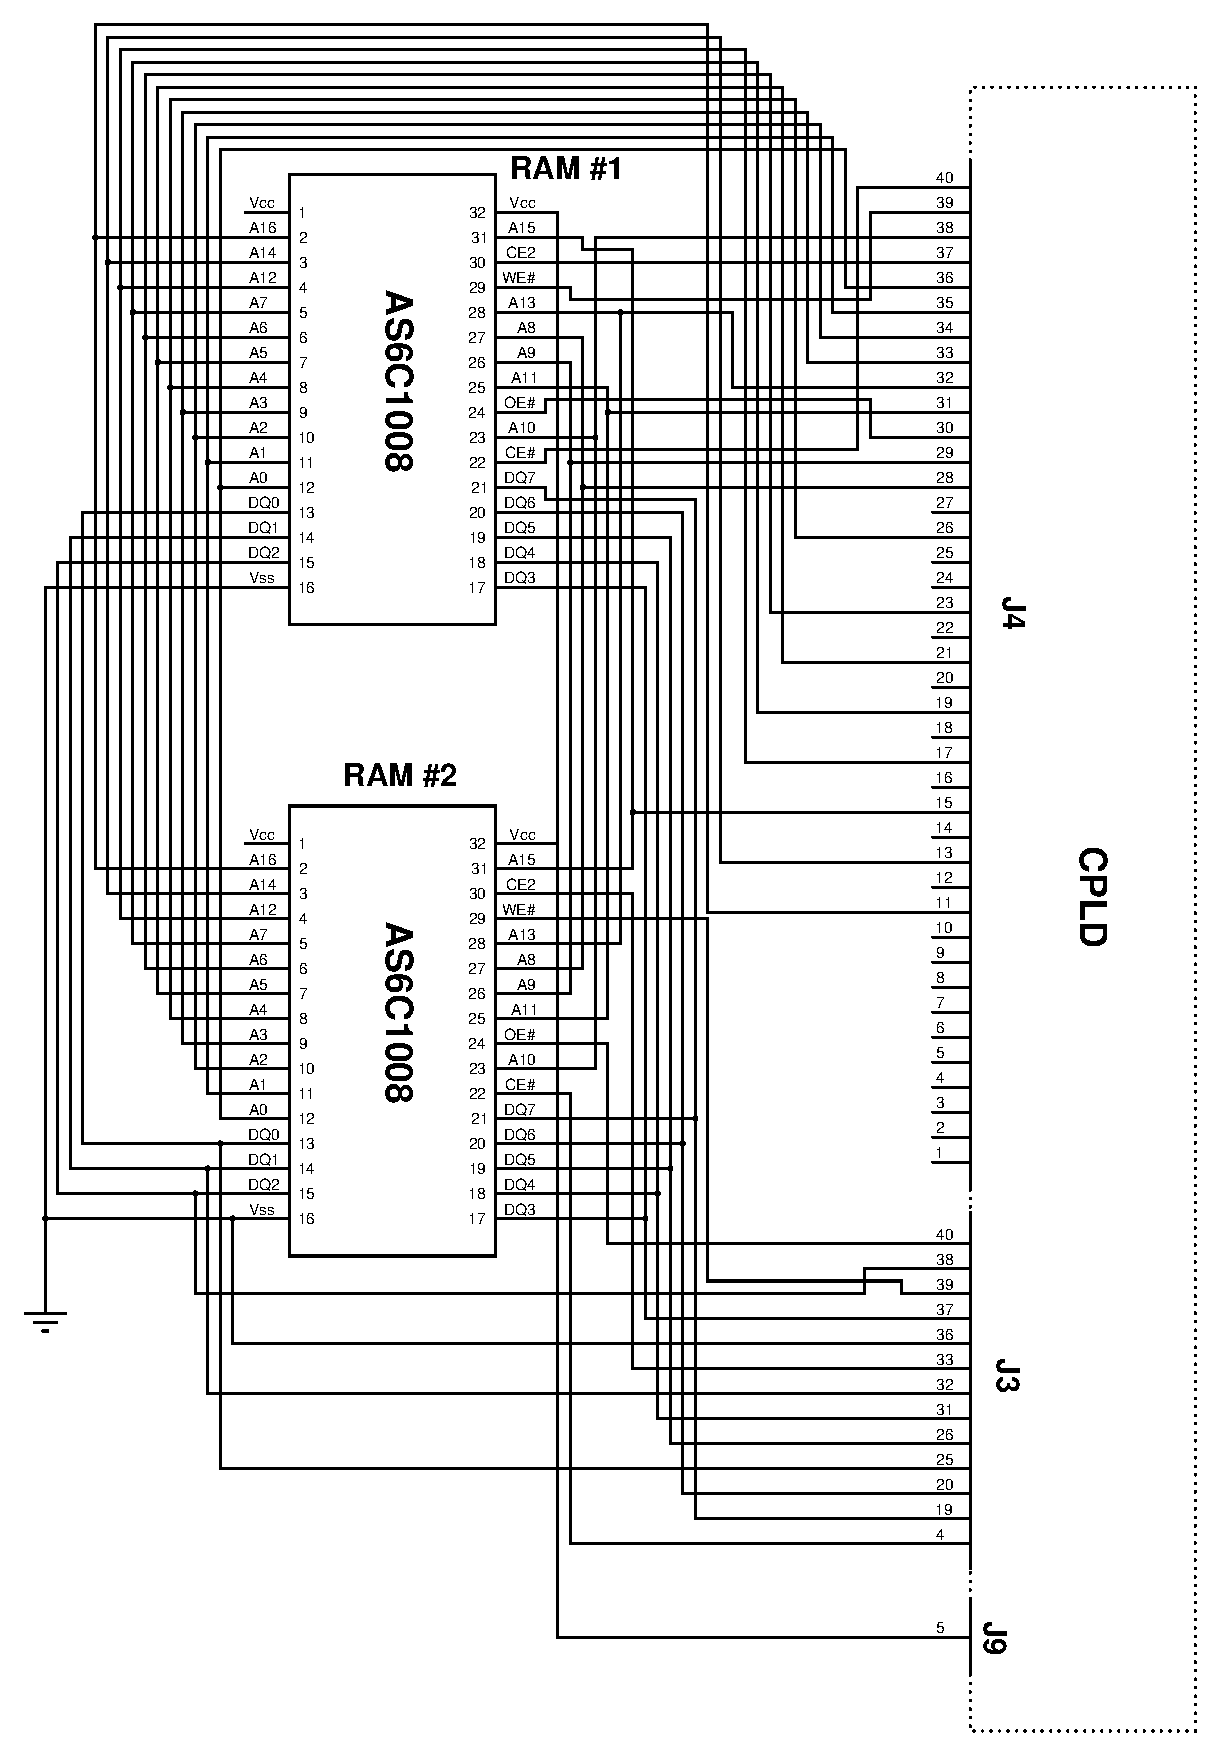
\includegraphics[scale=0.7]{figures/schematics/RAM_to_CPLD}
\caption{Schematic diagram of wires between both RAM chips and
the CPLD.}
\label{fig:ram_to_cpld}
\end{figure}

\begin{figure}
\center
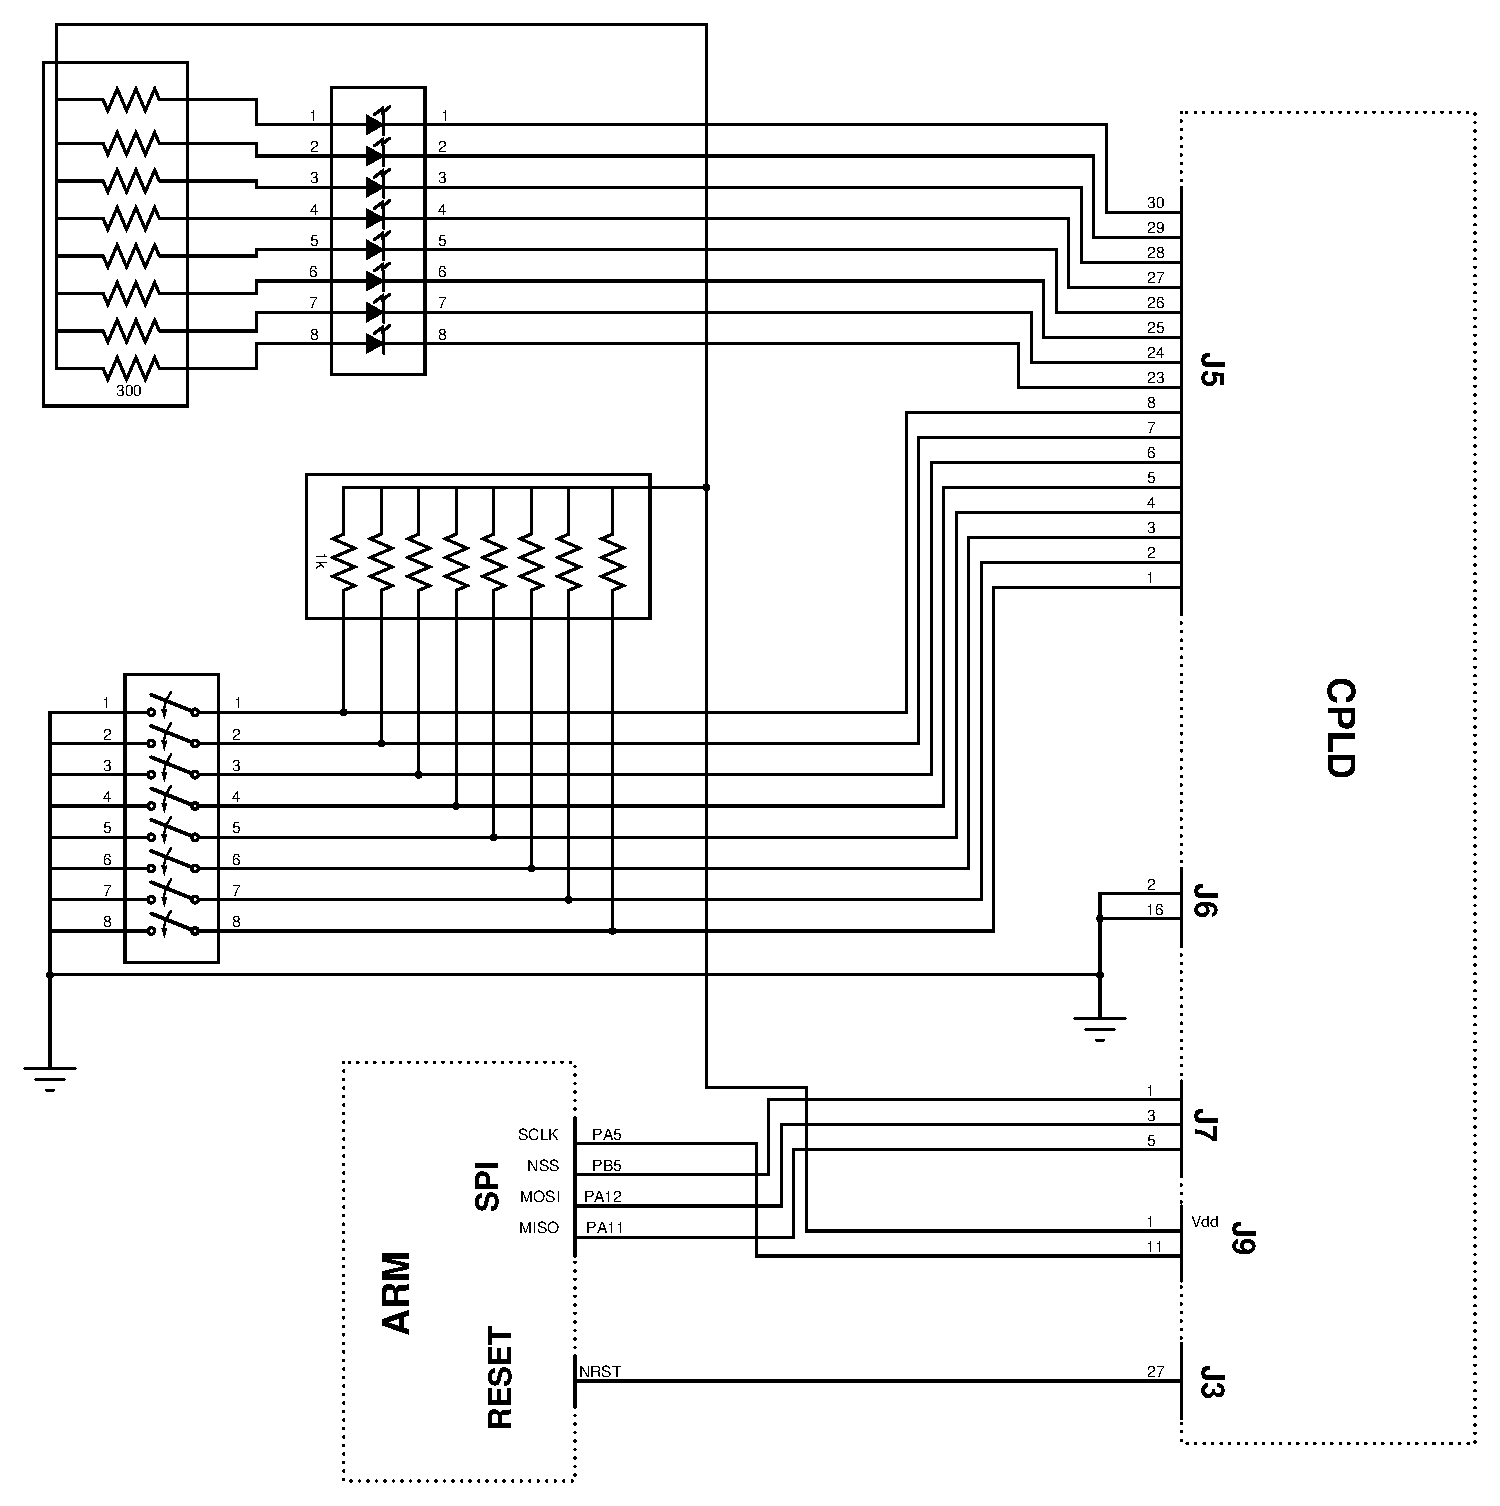
\includegraphics[scale=0.7]{figures/schematics/SPI_LEDs_SW}
\caption{Schematic diagram of wires between the ARM and the CPLD.}
\label{fig:arm_to_cpld}
\end{figure}

% {{{ pins Table
\begin{table}
	\center
	\begin{tabular}{|l|l|l|l|l|l|l|}
		\hline
		\multicolumn{7}{|c|}{\textbf{SPI}} \\
		\hline
		\multicolumn{1}{| c |}{\textbf{Verilog}} &
		\multicolumn{1}{| c |}{} &
		\multicolumn{1}{| c |}{\textbf{ARM}} &
		\multicolumn{4}{| c |}{\textbf{CPLD}} \\
		\hline
		name & description & pin  &  function & Mach XO Ball & Header & Pin \\
		\hline
		SCLK & SPI clock & PA5 & PT9B & D7 & J9 & 11 \\
		NSS & SPI slave select & PB5 & PR4C & F13 & J7 & 1 \\
		MOSI & SPI master out slave in & PA12 & PR4D & F12 & J7 & 3 \\
		MISO & SPI master in slave out & PA11 & PR5C  & B16 & J7 & 5 \\
		\hline
		\multicolumn{7}{|c|}{\textbf{switches}} \\
		\hline
		\multicolumn{1}{| c |}{\textbf{Verilog}} &
		\multicolumn{1}{| c |}{} &
		\multicolumn{1}{| c |}{\textbf{input switches}} &
		\multicolumn{4}{| c |}{\textbf{CPLD}} \\
		\hline
		name & description & pin  &  function & Mach XO Ball & Header & Pin \\
		\hline
		switches[0] & input switch 8 & 8 & PT2C & B2 & J5 & 1 \\
		switches[1] & input switch 7 & 7 & PT9A & D8 & J5 & 2 \\
		switches[2] & input switch 6 & 6 & PT2D & B3 & J5 & 3 \\
		switches[3] & input switch 5 & 5 & PT9C & E8 & J5 & 4 \\
		switches[4] & input switch 4 & 4 & PT3A & A2 & J5 & 5 \\
		switches[5] & input switch 3 & 3 & PT9D & E9 & J5 & 6 \\
		switches[6] & input switch 2 & 2 & PT3B & A3 & J5 & 7 \\
		switches[7] & input switch 1 & 1 & PT10A & A10 & J5 & 8 \\
		          & power, Vdd, pull up &      &     &    & J9 & 1 \\
		          & ground &  & & & J6 & 2 \\
		\hline
		\multicolumn{7}{|c|}{\textbf{LEDs}} \\
		\hline
		\multicolumn{1}{|c|}{\textbf{Verilog}} &
		\multicolumn{1}{|c|}{} &
		\multicolumn{1}{|c|}{\textbf{output LEDs}} &
		\multicolumn{4}{|c|}{\textbf{CPLD}} \\
		\hline
		name & description & pin  &  function & Mach XO Ball & Header & Pin \\
		\hline
%		bar\_leds[10] & output led 10 & 10 & PT5C & B4 & J5 & 21 \\
%		bar\_leds[9] & output led 9 & 9 & PT12A & A11  & J5 & 22 \\
		bar\_leds[0] & output led 8 & 8 & PT15D & B5   & J5 & 23 \\
		bar\_leds[1] & output led 7 & 7 & PT12B & A12  & J5 & 24 \\
		bar\_leds[2] & output led 6 & 6 & PT6E  & E7   & J5 & 25 \\
		bar\_leds[3] & output led 5 & 5 & PT12C & B11  & J5 & 26 \\
		bar\_leds[4] & output led 4 & 4 & PT6F  & E6   & J5 & 27 \\
		bar\_leds[5] & output led 3 & 3 & PT12D & B12  & J5 & 28 \\
		bar\_leds[6] & output led 2 & 2 & PT16C & A5   & J5 & 29 \\
		bar\_leds[7] & output led 1 & 1 & PT13C & C11  & J5 & 30 \\
		          & power, Vdd, pull up &      &     &    & J9 & 1 \\
		          & ground &  & & & J6 & 16 \\
		\hline
		\multicolumn{7}{|c|}{\textbf{reset}} \\
		\hline
		\multicolumn{1}{| c |}{\textbf{Verilog}} &
		\multicolumn{1}{| c |}{} &
		\multicolumn{1}{| c |}{\textbf{ARM}} &
		\multicolumn{4}{| c |}{\textbf{CPLD}} \\
		\hline
		name & description & pin  &  function & Mach XO Ball & Header & Pin \\
		\hline
		reset\_n & active low reset & NRST & PL7B & G2 & J3 & 27 \\
		\hline
	\end{tabular}
	\caption{Definition of the pin assignments between the ARM board,
		the CPLD, and other devices.
        Notice that the switch and LEDs are reversed.
        This was done so that the orientation from LSB to MSB is from
        right to left.
        }
	\label{tbl:pins}
\end{table}
% }}}

% configuring using Diamond
In Diamond the pins were configured with standard options:
low voltage 3.3 volt CMOS with no pull up or pull down.
Output pins to drive the leds were configured for 8 mA drive current.

% input switches
The input switches to the CPLD can be interfaced by connecting
one end to ground and the other end to the pin along with a
pull up resistor to Vdd.
A resistor value between 1k and 10k should be acceptable.
And the pull up voltage for Vdd can be sourced from a pin on
the board (Table \ref{tbl:pins}).

% output leds
The output LEDs are connected to the CPLD using a series
resistor.
Vdd would connect to the resistor which connects to the led
(forward biased) which connects to the pin.
The value of the resistor should limit the current to approximately
10 mA.
A value of 300 $\ohm$ is a typical value.

% reset pin
To reset the boards their reset pins must be configured.
The ARM board provides a \verb+NRST+ pin which is at Vcc
when enabled and goes low when the reset button is pushed\cite[Pg. 17, 20]{UM1079}.
This can then be connected to the CPLD to cause
it to reset using \verb+GSRN+\citetext{\citealp[Pg. 13, 46, 50, 53]{DS1002}; \citealp[Pg. 8]{EB66}}.
Table \ref{tbl:pins} lists the pins that were used.

\clearpage

% }}}

% {{{ Development
\section{Development}

While the end result of this project is simple its development
was far from easy.

% sythesis
All the code to control the CPLD was written in Verilog.
While Verilog is a rich language with numerous
capabilities\cite{thomas2002verilog} only a small fraction of it
can be synthesized in to functional code.
It was often trivial to devise a solution
but the code had to be significantly reworked in order to get it to
synthesize\footnote{The term "synthesize" is used to describe when
the Verilog code is processed under strict rules by a program such
as Diamond or Synplify.  Simulating the code under Icarus Verilog
is not considered "synthesizing" because it is far less strict.}.

As an example of one of one of the common synthesis problems,
suppose it was desired to increment a variable on the rising
edge and falling edge of a clock.
The Verilog simulator (Icarus) will allow this and it will simulate
properly.
But this code can't be synthesized because it can't be turned in to a flip flop.

As another example, suppose it was desired to reset all the variables on
a falling edge of the NSS signal, and then mutate the variables during
subsequent rising edges of the SCK signal.
Again this will simulate properly but it cannot be synthesized because
two different always blocks cannot modify the same variable.

% debugging
Beyond synthesis errors there seemed to be an endless supply of problems
which were quite intricate and difficult to diagnose.
Without a full arsenal of debugging techniques this project is nearly impossible.
For the simple problems "trial and error" could be used but more
often this was impractical.
A logic analyzer with a minimum of four channels was invaluable for
diagnosing errors with SPI communications such as glitches and shifts.
A C debugger was crucial for stepping through the ARM code
to verify that it is behaving as expected.

An example of one of the problems that had to be diagnosed were
glitches on the SPI.
This normally first appears as incorrect or erratic values being
received by the master (MISO).
Using a logic analyzer this problem can be clearly seen by spikes
which rise and fall at a single clock edge.
If it is operating normally it should only rise or fall at a single clock edge.
The next logical step was to investigate the CPLD since it is driving the
output.
With the MISO signal wire disconnected from the ARM it will be seen that
the wire is being driven properly and there are no glitches.
But how can the ARM disrupt the signal if it is only an input?
While it is not exactly clear how this signal is disrupted, it is caused
by the GPIO sample speed being configured for too slow of a speed.
A trial and error approach to this problem would have been nearly impossible.
Only by using a methodical approach along with the proper tools was this
problem able to be solved in a practical amount of time.

% }}}

% {{{ Conclusion
\section{Conclusion}
% difficulties

% was it a success?
While this project was a success in creating bus communications over SPI
its development was far more difficult than expected.
Writing synthesizeable Verilog code and debugging the numerous intricate
problems were the biggest hindrances to a timely completion of this project.

% }}}

% {{{ References
\clearpage

\pagebreak
\renewcommand*{\refname}{\vspace{-8mm}}
\section{References}
%\bibliographystyle{ieeetr}
\bibliographystyle{plain}
\bibliography{references}
% }}}

\end{document}

% vim:foldmethod=marker

